\documentclass[12pt,oneside,a4paper,english]{article}
\usepackage[utf8]{inputenc} 
\usepackage[T1]{fontenc}
\usepackage[margin=2cm,headheight=20pt,includeheadfoot]{geometry}
\setlength{\textfloatsep}{10pt plus 1.0pt minus 2.5pt}
\setlength{\headsep}{9pt}
\usepackage[english]{babel}
\usepackage{listings}
\usepackage{color}
\usepackage{titlesec}
\usepackage{titling}
\usepackage[framed, numbered]{matlab-prettifier}
\usepackage{changepage}
\usepackage{amsmath}
\usepackage[hidelinks]{hyperref}
\usepackage{enumitem}
\usepackage{graphicx}
\usepackage{fancyhdr}
\usepackage{lastpage}
\usepackage{caption}
\usepackage{tocloft}
%Change numbers to letters
%\renewcommand\thesubsection{\alph{subsection}}
\usepackage{setspace}
\usepackage{multirow}
\usepackage{titling}
\usepackage{float}
\usepackage{comment}
\usepackage{booktabs}
\usepackage{indentfirst}
\usepackage{lscape}
\usepackage{booktabs,caption}
\usepackage[flushleft]{threeparttable}
\usepackage[english]{nomencl}
\usepackage{xcolor}
\usepackage{lipsum}
\usepackage{amsfonts}
\usepackage{mathtools}
\usepackage[section]{placeins}
\usepackage{siunitx}
\usepackage{todonotes}
\usepackage[inkscapelatex=false]{svg}
\usepackage{matlab-prettifier}
\usepackage{float} % die folgenden drei packages sind für die Darstellung von Grafiken bzw. mehreren Grafiken mit einer gesamten Caption
\usepackage{subfigure}
\usepackage{wrapfig} %Bild im Text
\usepackage{nicefrac}
\usepackage{titlesec}
\usepackage{graphicx}
\usepackage{makecell} % in der Präambel
\usepackage{tabularx}
\usepackage{subcaption}


% --- set footer and header ---
\pagestyle{fancy}
\fancyhf{}

\setlength{\parindent}{2em}
\title{Analysis of measured wind dataa} % to reference as \title, dont use \maketitle
\makeatletter\let\Title\@title\makeatother

\lstset{language=Matlab,
style=Matlab-editor,
basicstyle=\normalsize\mlttfamily,
numbers=left,
numberstyle={\scriptsize\color{black}},			% size of the numbers
numbersep=0.5cm											
}

\newlist{steps}{enumerate}{1}
\setlist[steps, 1]{leftmargin=1.5cm,label = Step \arabic*:}
\renewcommand{\headrulewidth}{1pt}
\renewcommand{\footrulewidth}{1pt}

%\lhead{\Title}

\lhead{\Title}
\rfoot{
\includegraphics[height=1.25cm]{root/logo.pdf}} % right header logo
\setlength\headheight{16pt}
\setlength{\footskip}{50pt}
\lhead{\Title} %rightH title
\cfoot{\thepage}

% --- End of page settings ---

\lstdefinestyle{MatlabStyle}{
    language=Matlab,
    basicstyle=\ttfamily\footnotesize,
    keywordstyle=\color{blue},
    commentstyle=\color{green!50!black},
    stringstyle=\color{red},
    numbers=left,
    numberstyle=\tiny,
    stepnumber=1,
    numbersep=5pt,
    frame=single
}


\begin{document}
\titlespacing{\section}{0pt}{*2}{*0.5}
\pagenumbering{roman} 
\input{sources/0_frontpage.tex}

\newpage
\doublespacing
%\addcontentsline{toc}{section}{Table of Contents}
\renewcommand{\baselinestretch}{1}\normalsize
\tableofcontents
\renewcommand{\baselinestretch}{1}\normalsize
%\singlespacing
\thispagestyle{fancy} % force page style

%\newpage
%\addcontentsline{toc}{section}{List of Figures}
%\fancyfoot[C]{Page \thepage\ of \pageref{LastPage}}
%\listoffigures
%\thispagestyle{fancy}

\newpage
\pagenumbering{arabic} 
\fancyfoot[C]{Page \thepage\ of \pageref{LastPage}}
\setlength{\parindent}{0pt}

\section{Part 1: Vertical variation of wind speed}
\label{sec:part1}

\subsection{Met Mast and Location}
\textbf{Task:} Describe the met mast and its location. How do the surroundings of the mast look in terms of terrain roughness? How far is the mast from the turbine and in which direction? Why?

The measurements are from DTU Risø Campus using a met mast with a total height of 70 m. The mast is around 120 m, away from the Vestas V52 wind turbine.
The surrounding terrain has a low roughness to the west  (due to water from the Roskilde Fjord) and a higher roughness in the other directions since it consists of open fields and the campus buildings.
To assure the free flow, the mast is posi
% Hier Text einfügen

\subsection{Data Collection}
\textbf{Task:} Describe the data collected. What has been measured, what units, what sample rate, where at the mast and with what instruments?

\subsection{Raw Time Series Plot}
\textbf{Task:} Plot the raw time series of the wind speed at the different heights. What time scales do you see? Do they differ for the different heights?

\begin{figure}[H]
    \centering
    % \includegraphics[width=0.8\textwidth]{figures/Q3_plot.png}
    \caption{Raw wind speed time series at various heights (10th Feb 2026).}
\end{figure}

\subsection{Logarithmic Wind Profile}
\textbf{Task:} Plot the average wind speed for each height against height $z$. Can the profile be described by a logarithmic wind profile?

\subsection{Roughness Length and Friction Velocity}
\textbf{Task:} Estimate the roughness length $z_0$ and the friction velocity $u_*$ from the observed wind profile.

\subsection{Stability Impact}
\textbf{Task:} Discuss the validity of the logarithmic profile under the observed stability conditions.

\subsection{Heat Flux and Stability}
\textbf{Task:} Estimate the friction velocity and the heat flux from the sonic anemometer data.

\subsection{Weather Conditions}
\textbf{Task:} How was the weather at the day of visit? Does the observed weather support your finding of question 7?


The day we visited Risø was windy from the eastern direction with some snowflakes. Generally, the site experiences western winds from the fjord, but that was not the case that day.

\textcolor{red}{does it support finding of Q7?}

\section{Part 2: Statistical analysis of multi-year wind climate}
\label{sec:part2}

\subsection{Data Description}
\textbf{Task:} Describe the data. What has been measured, in what units, at which locations, with which instruments and with what temporal resolution?

The dataset consists of eight years of wind observations from 2018 to 2026, provided as 10-minute mean values. 
The data in the file \texttt{tenMinutesData\_2018\_2024.csv} originates from the meteorological mast at the DTU Risø Campus.

\begin{table}[H]
    \centering
    \begin{tabular}{llll}
        \toprule
        \textbf{Parameter} & \textbf{Symbol} & \textbf{Unit} & \textbf{Instruments / Label} \\
        \midrule
        Wind speed & sp & [m/s] & Cup (W) and Sonic (SW) anemometers \\
        Wind direction & dir & [$^\circ$] & Wind vanes (W) and Sonic (SW) sensors \\
        Precipitation & Rain & [mm] & Tipping bucket rain gauge \\
        \bottomrule
    \end{tabular}
    \caption{Summary of measured parameters and sensor types.}
\end{table}

The measurements are available at specific heights, including 57 m and 70 m for wind speed, and 41 m for wind direction. For the long-term climate analysis and the Annual Energy Production (AEP) calculation of the V52 turbine, the data collected at the 70 m height is of primary interest.

\subsection{Raw Data and Gaps}
\textbf{Task:} Plot the raw data as function of time. Identify any data gaps and discuss possible reasons for these gaps.

\subsubsection{Time Series Visualization}
The raw 10-minute average data for wind speed, direction, and precipitation is plotted for the period between 2018 and 2026. This includes measurements from cup anemometers, sonic anemometers, and wind vanes at various heights.

\begin{figure}[H]
    \centering
    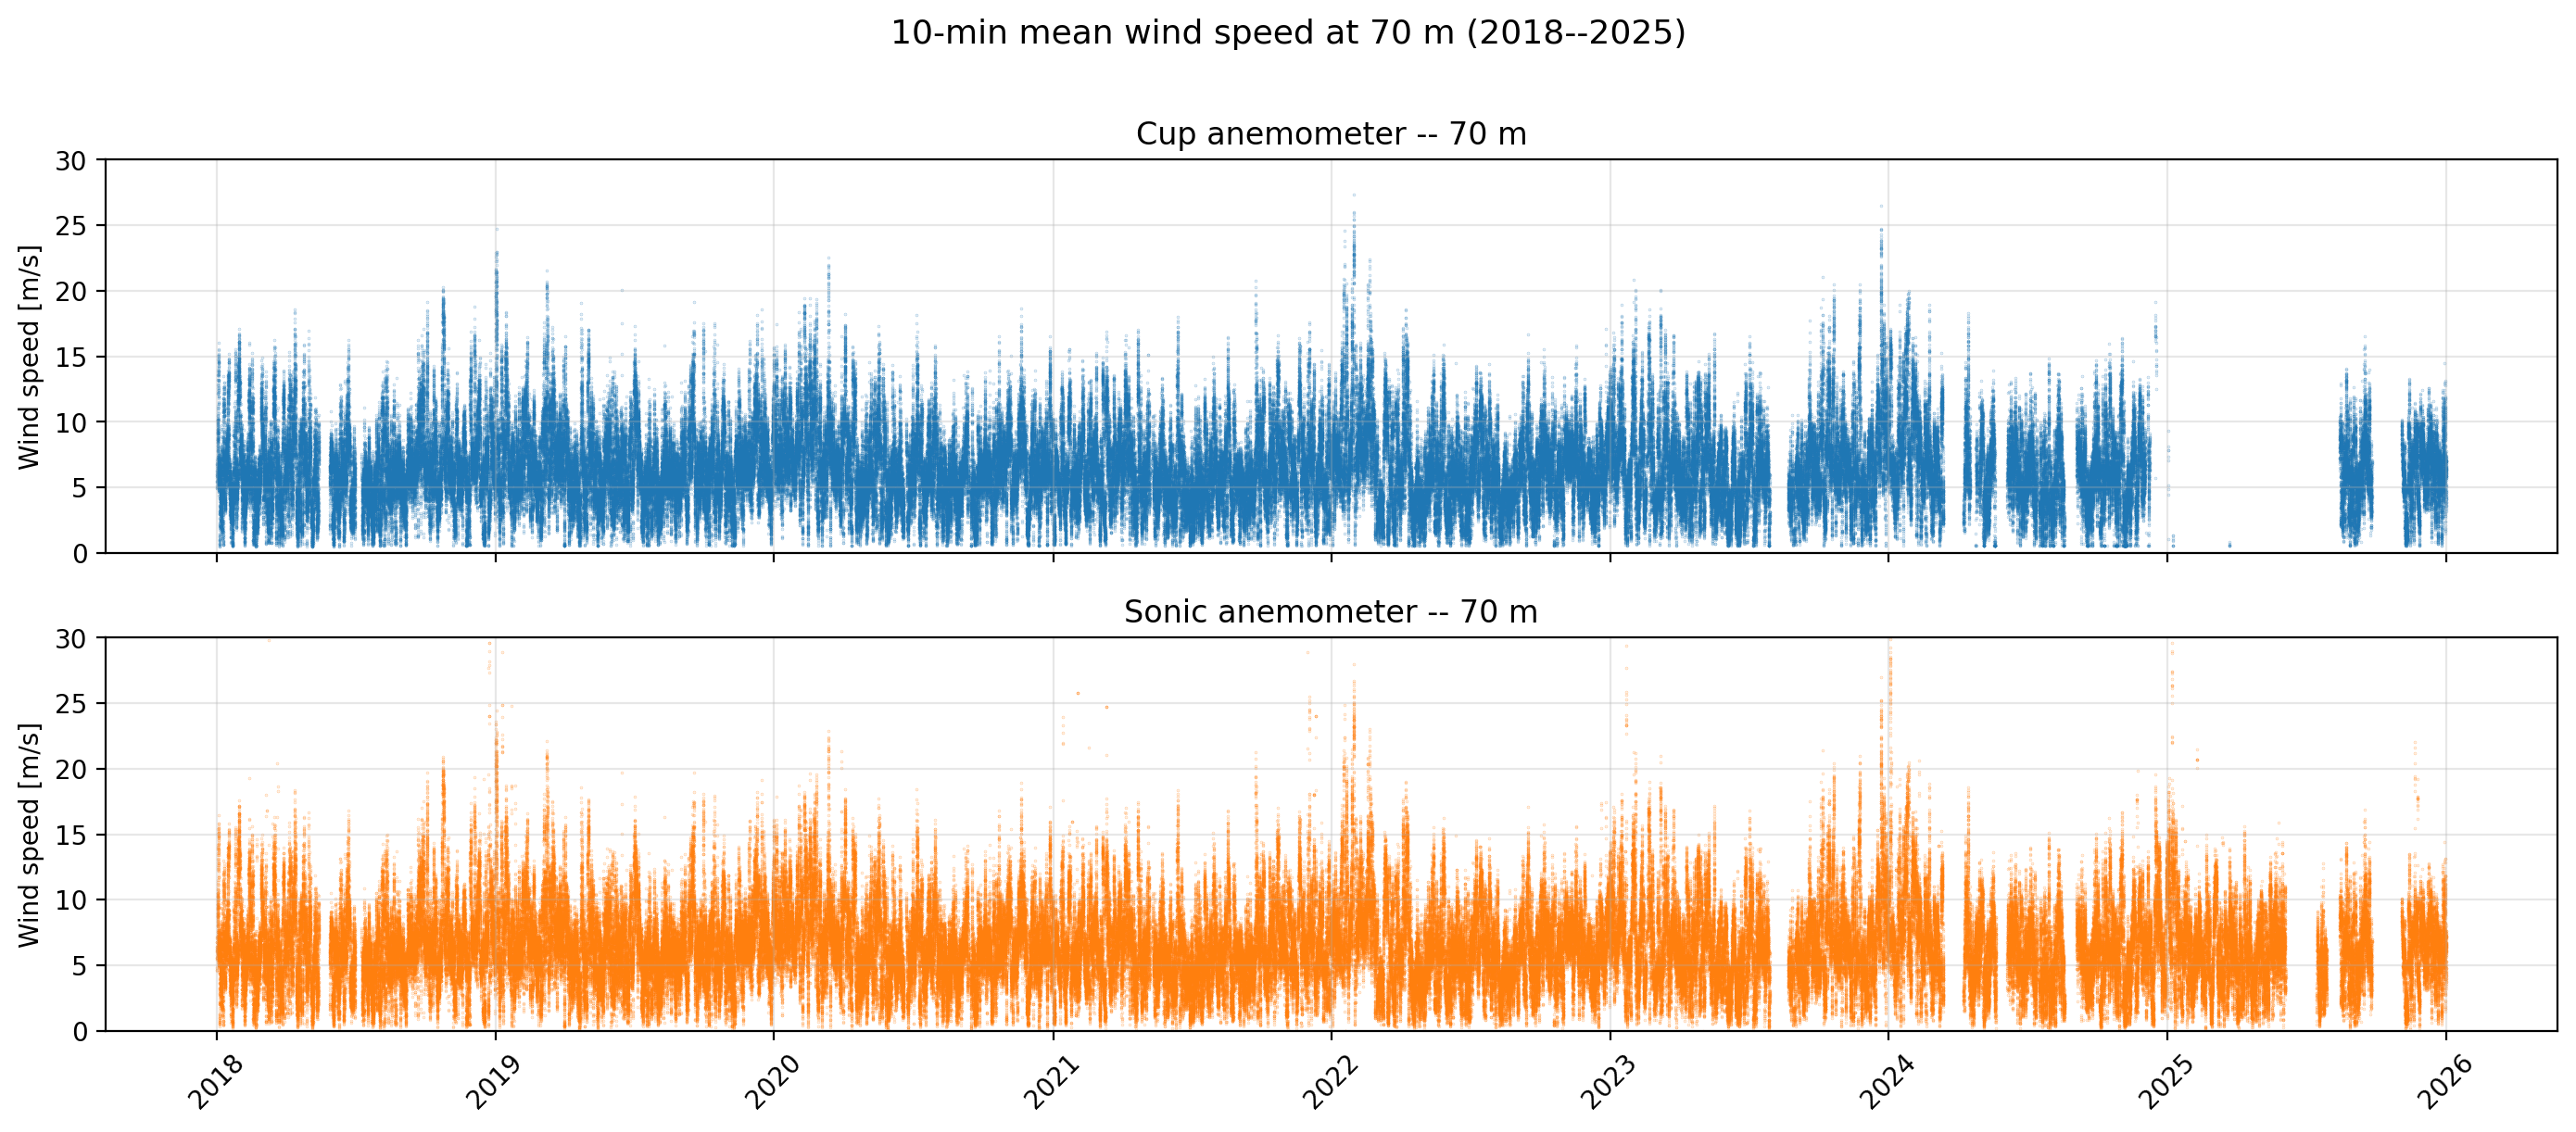
\includegraphics[width=1\textwidth]{figures/Q10_Wsp_70m.png}
    \caption{Raw 10-minute wind speed at 70m comparing Cup and Sonic anemometers.}
\end{figure}

\begin{figure}[H]
    \centering
    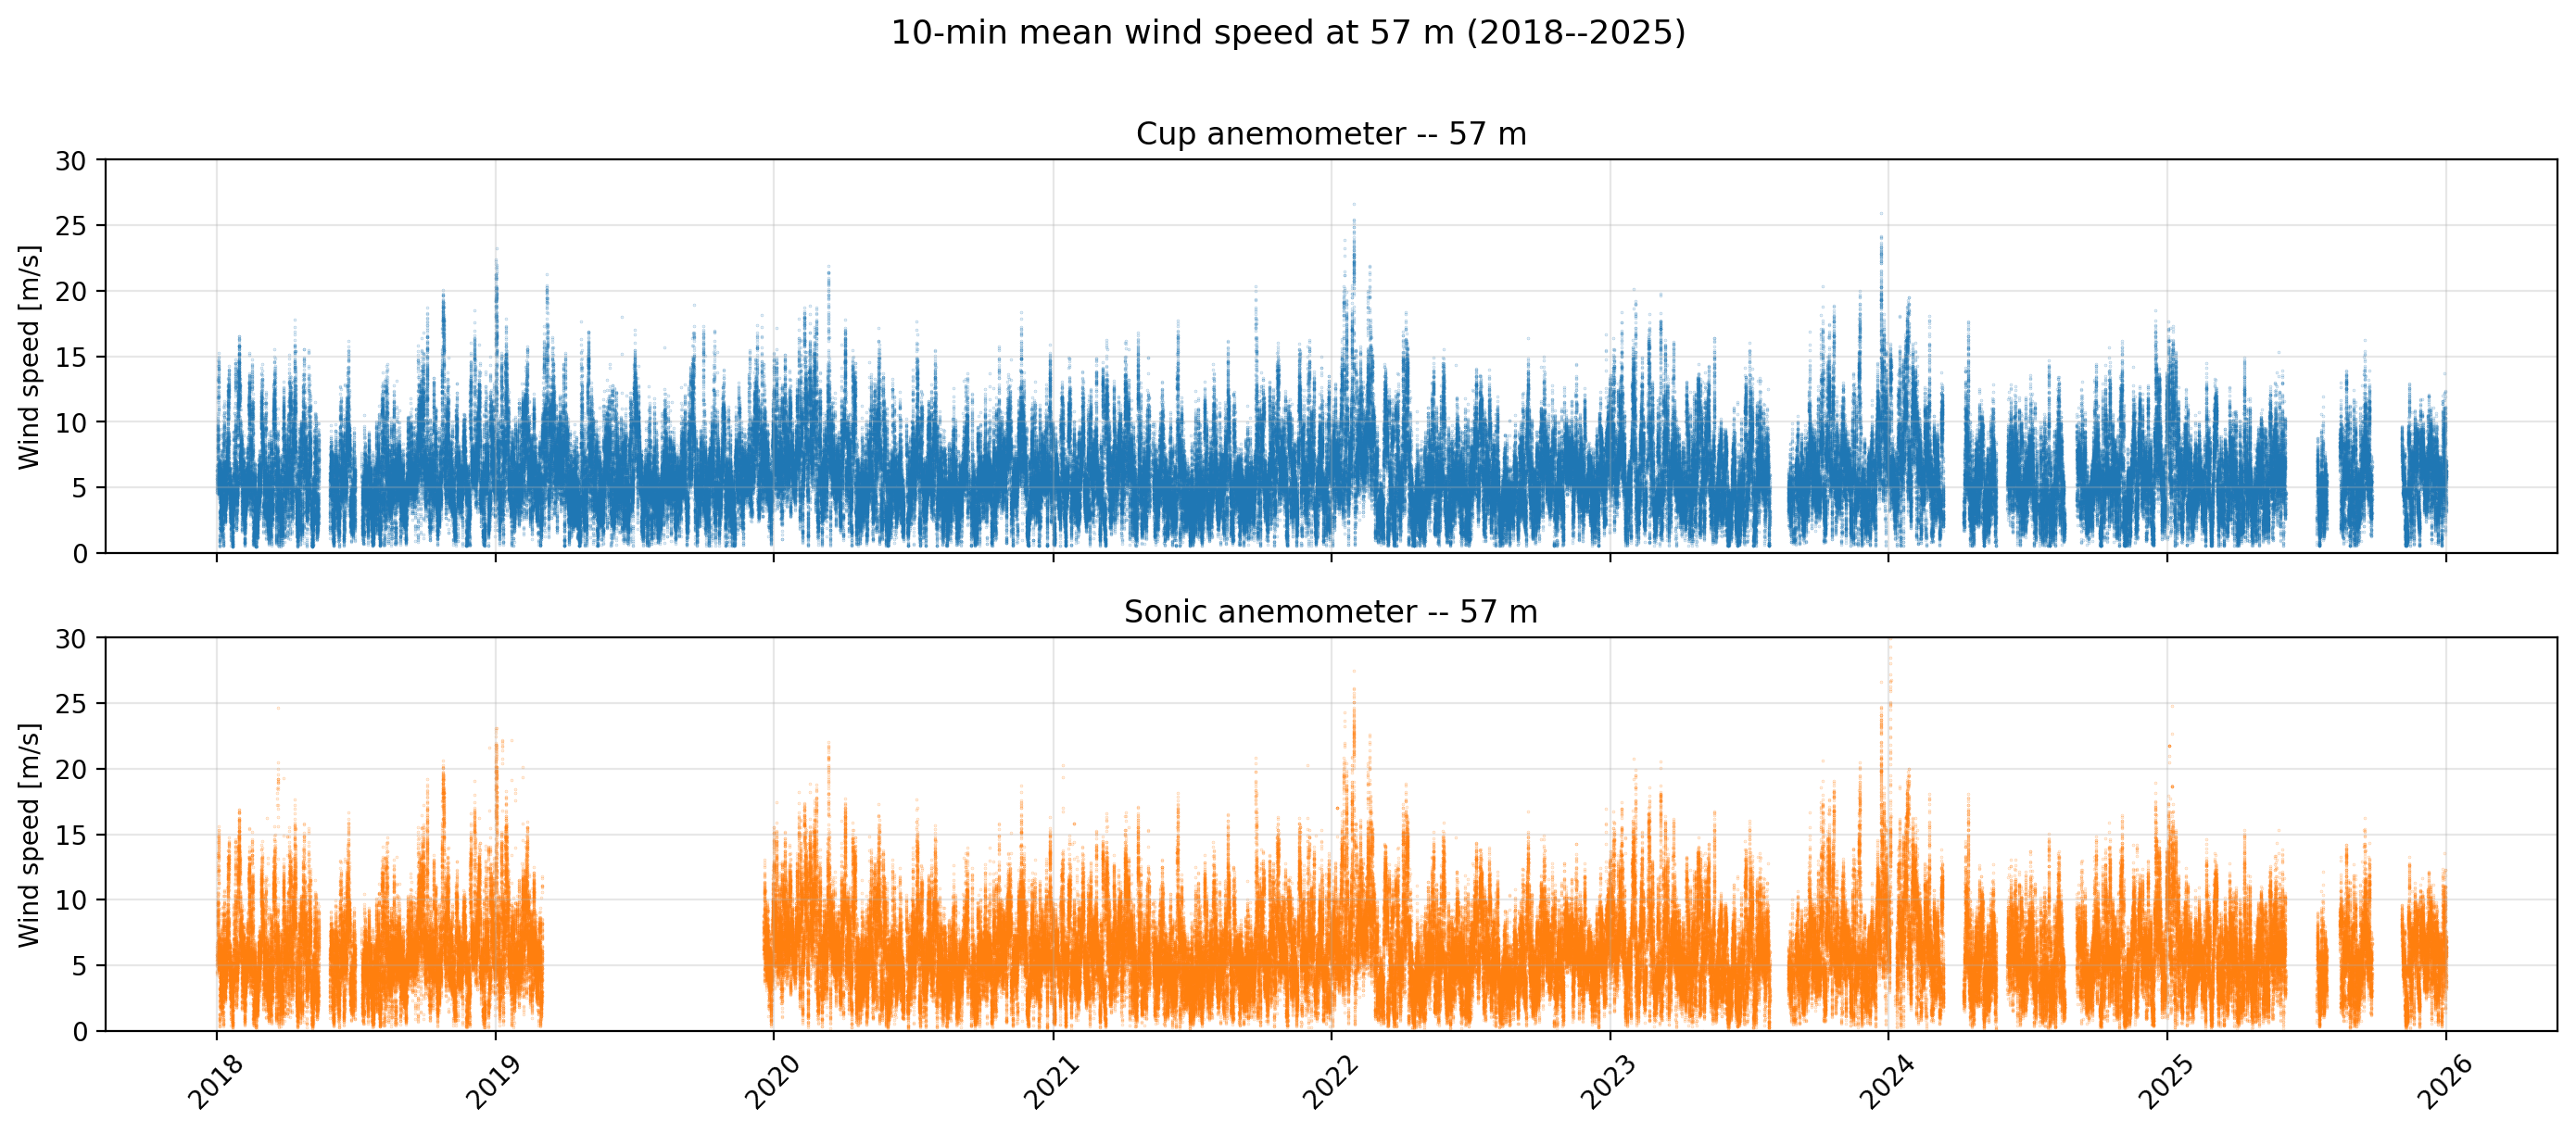
\includegraphics[width=1\textwidth]{figures/Q10_Wsp_57m.png}
    \caption{Raw 10-minute wind speed at 57m comparing Cup and Sonic anemometers.}
\end{figure}
\begin{figure}[H]
    \centering
    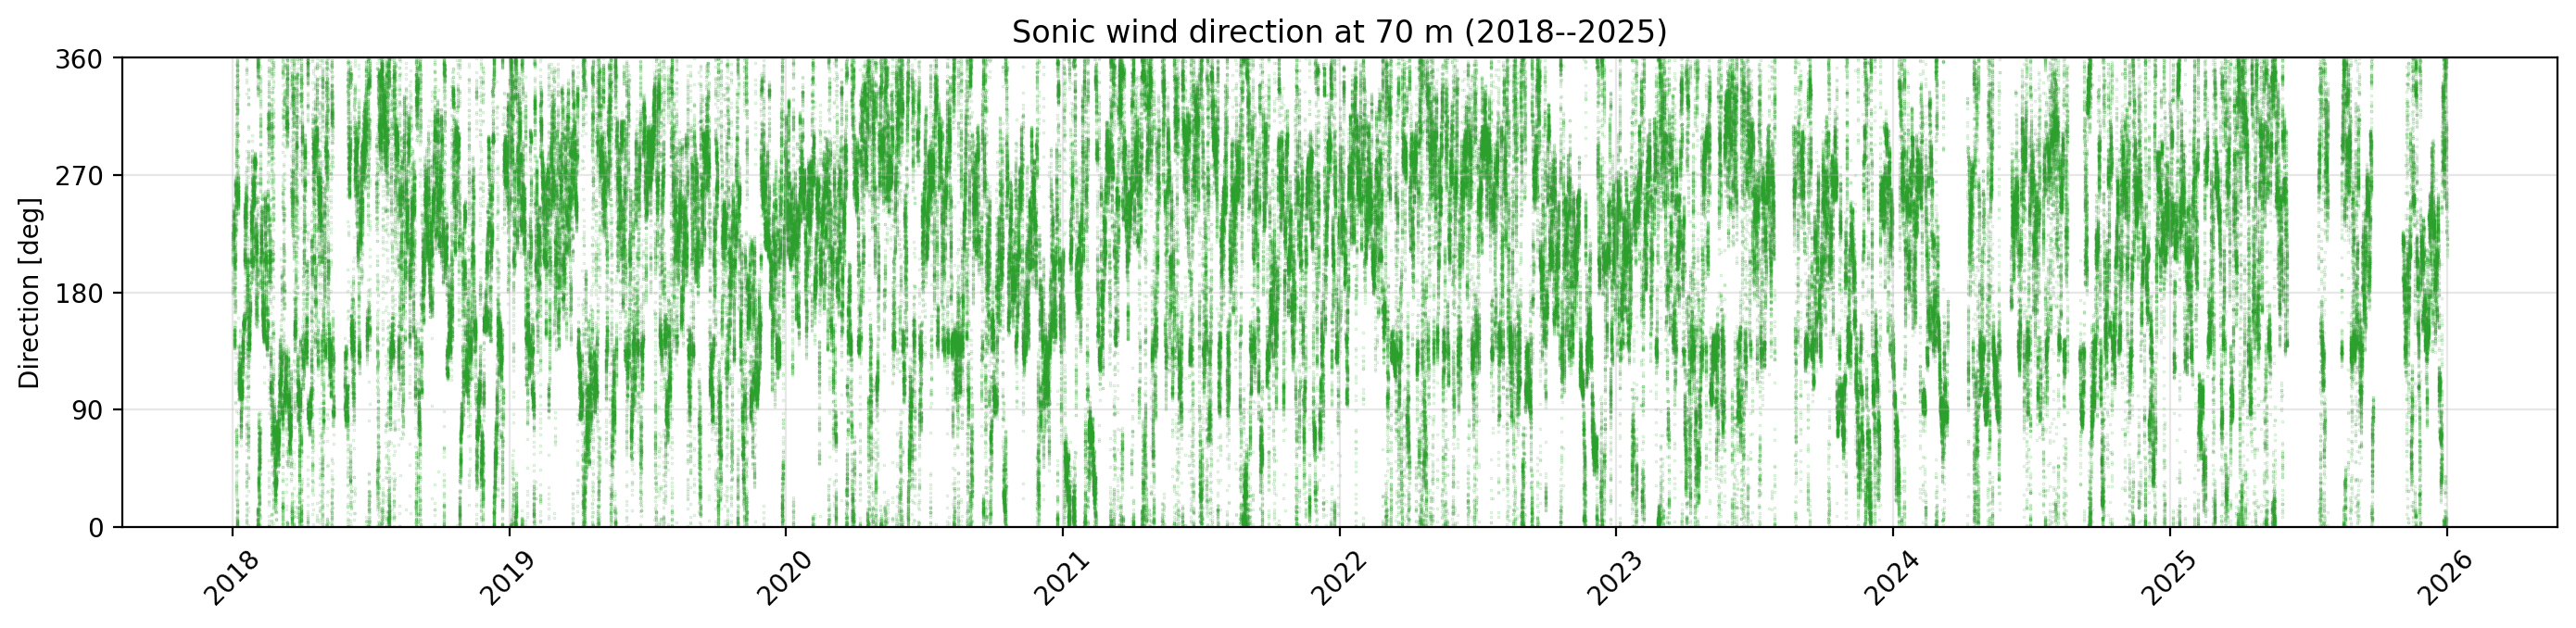
\includegraphics[width=1\textwidth]{figures/Q10_Dir_70m.png}
    \caption{Wind direction time series from the Sonic anemometer at 70m height.}
\end{figure}

\begin{figure}[H]
    \centering
    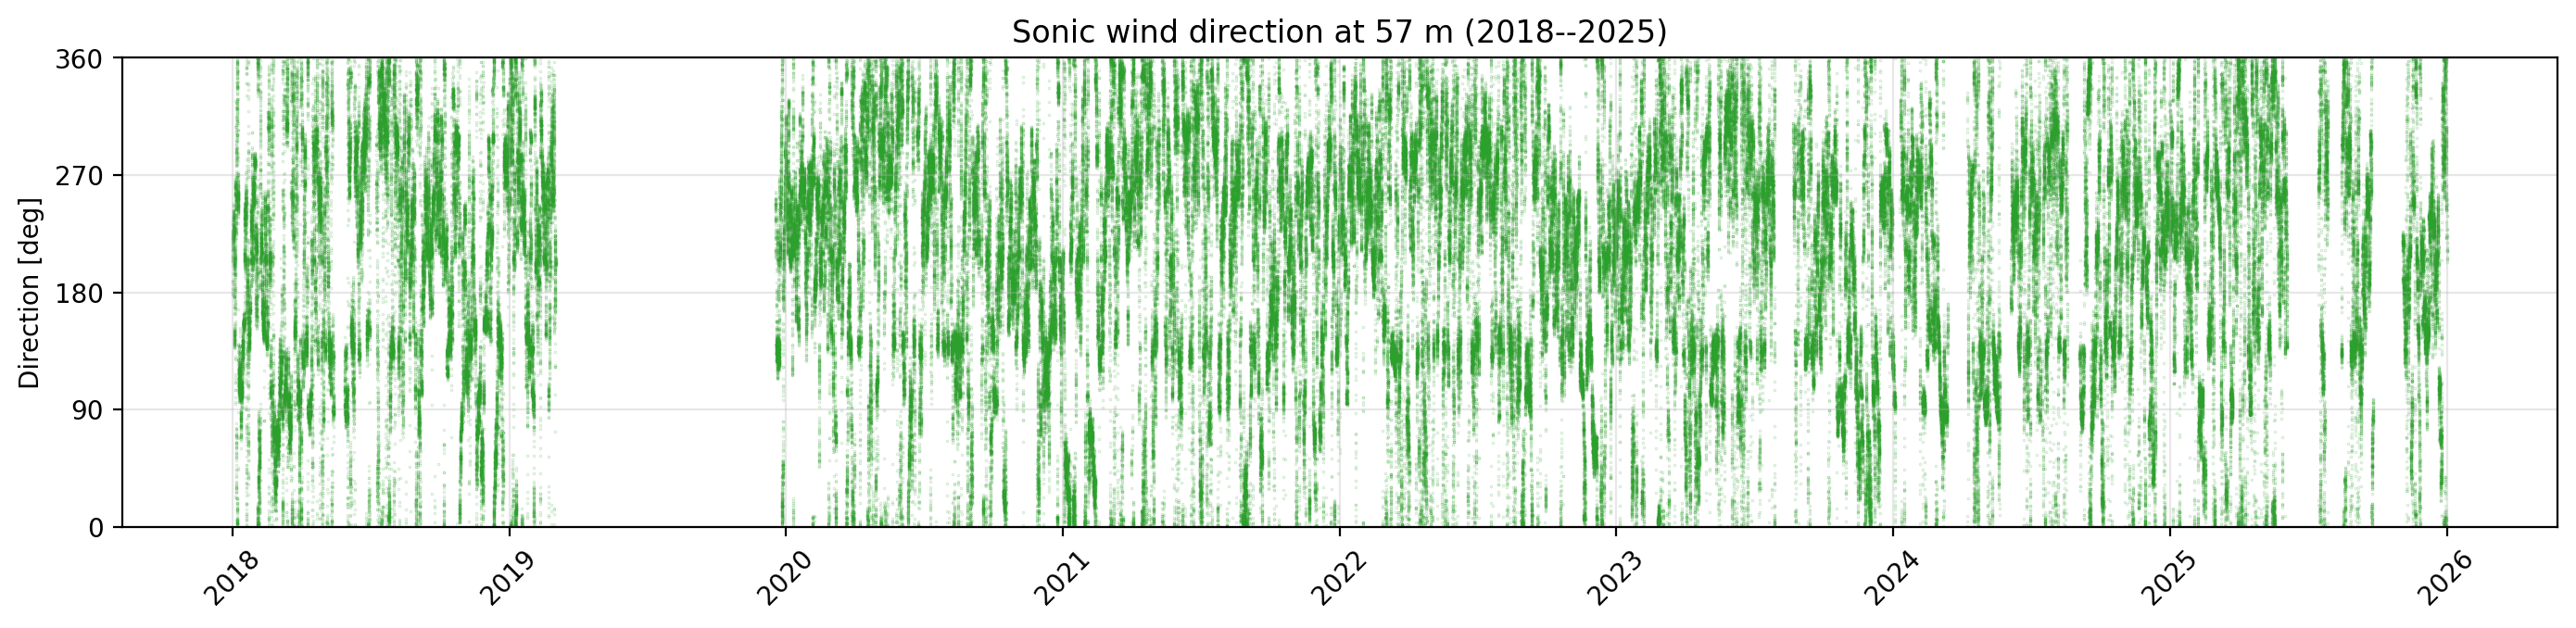
\includegraphics[width=1\textwidth]{figures/Q10_Dir_57m.png}
    \caption{Wind direction time series from the Sonic anemometer at 57m height.}
\end{figure}

\begin{figure}[H]
    \centering
    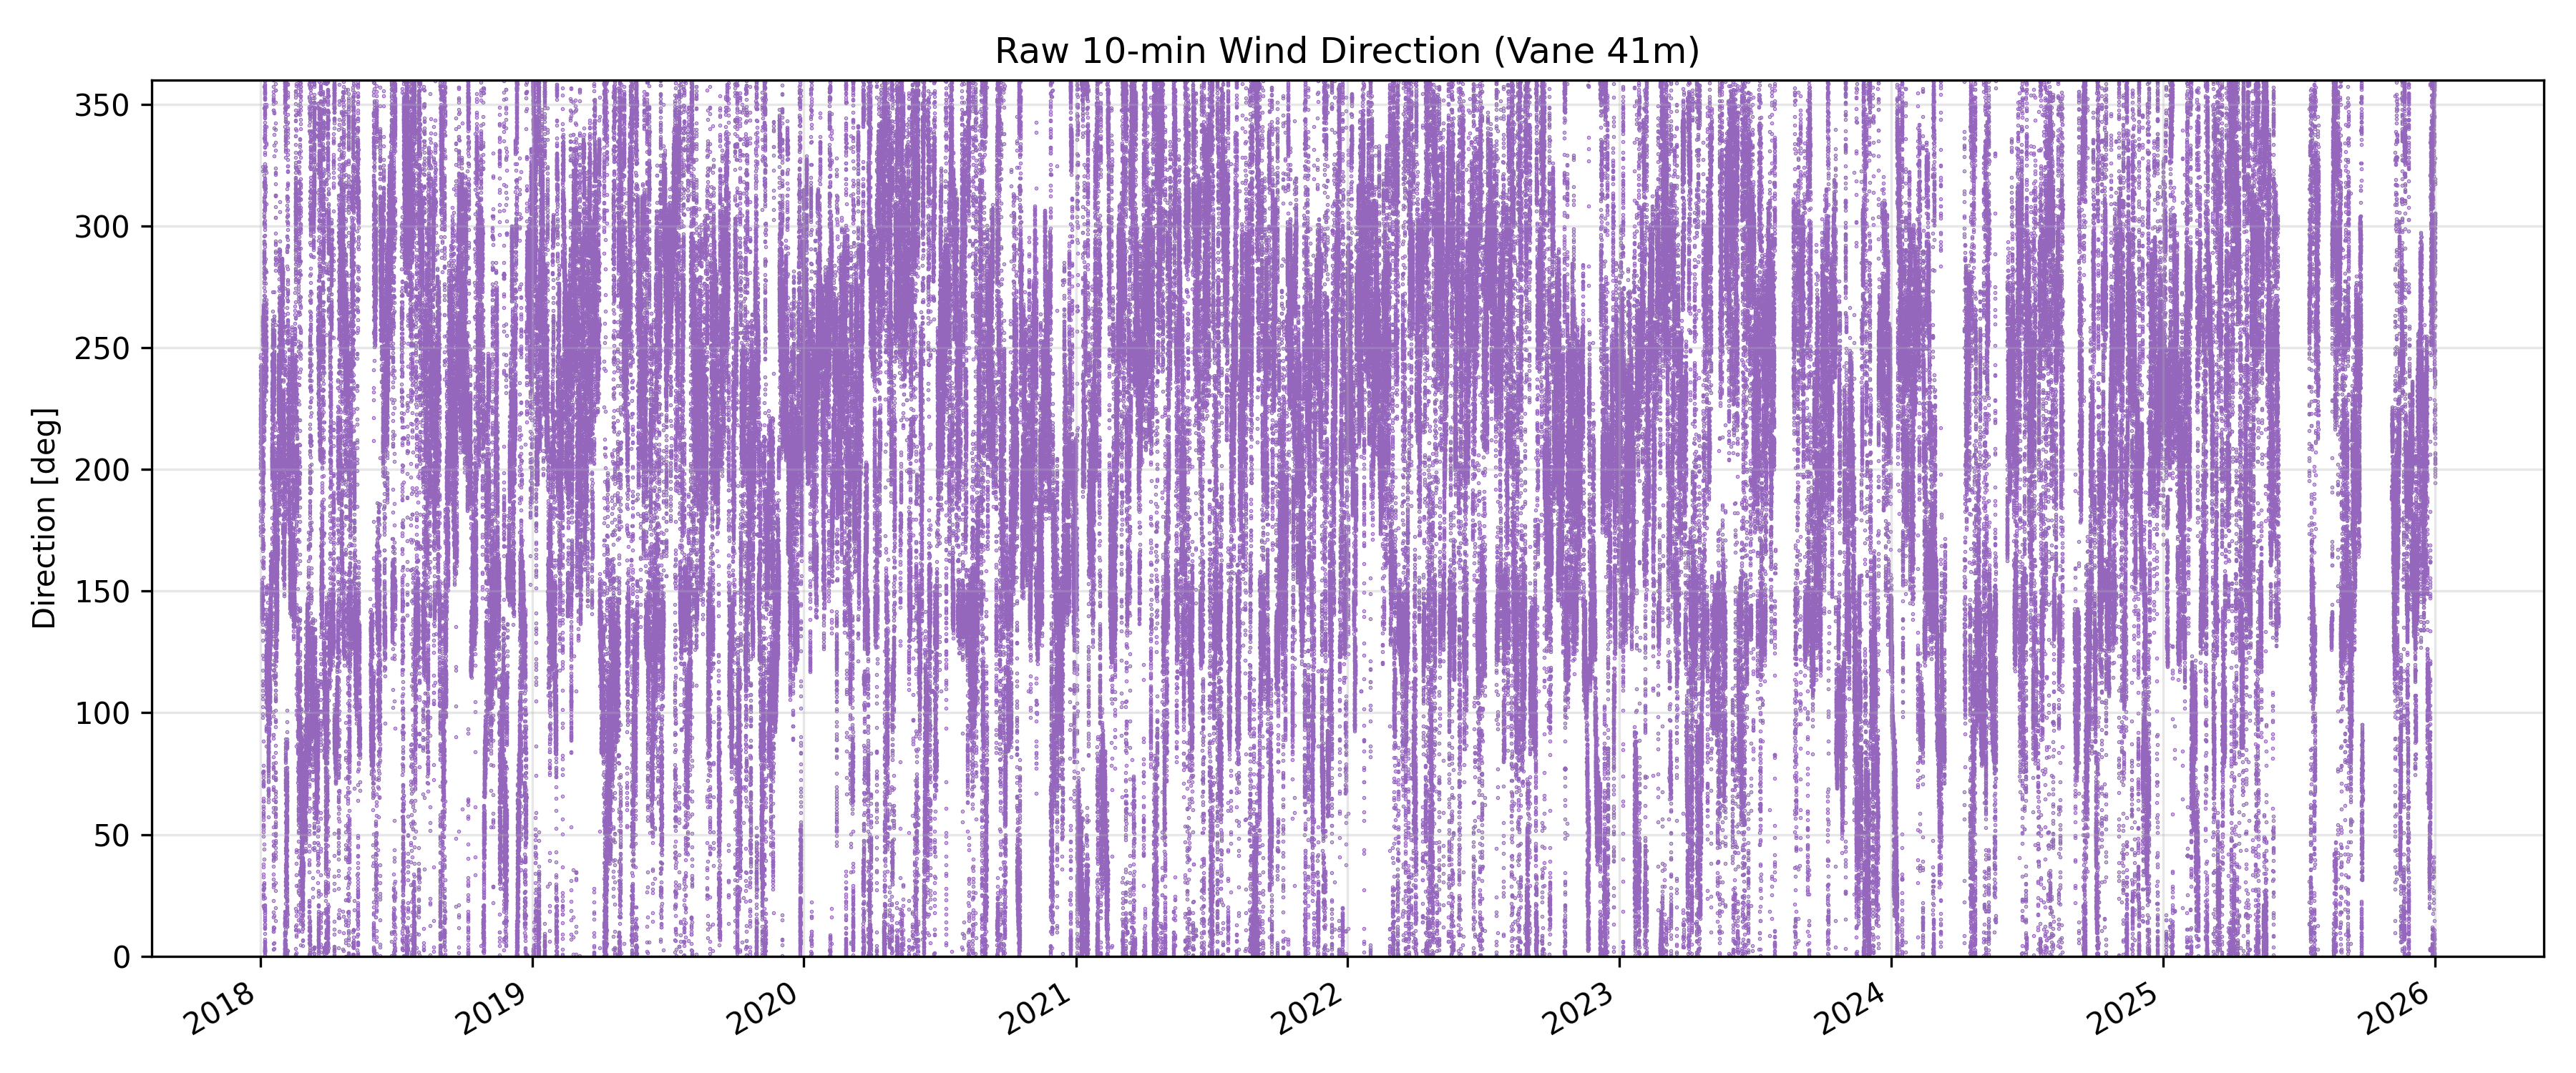
\includegraphics[width=1\textwidth]{figures/Q10_Dir_41m.png}
    \caption{Wind direction time series from the wind vane at 41m height.}
\end{figure}

\begin{figure}[H]
    \centering
    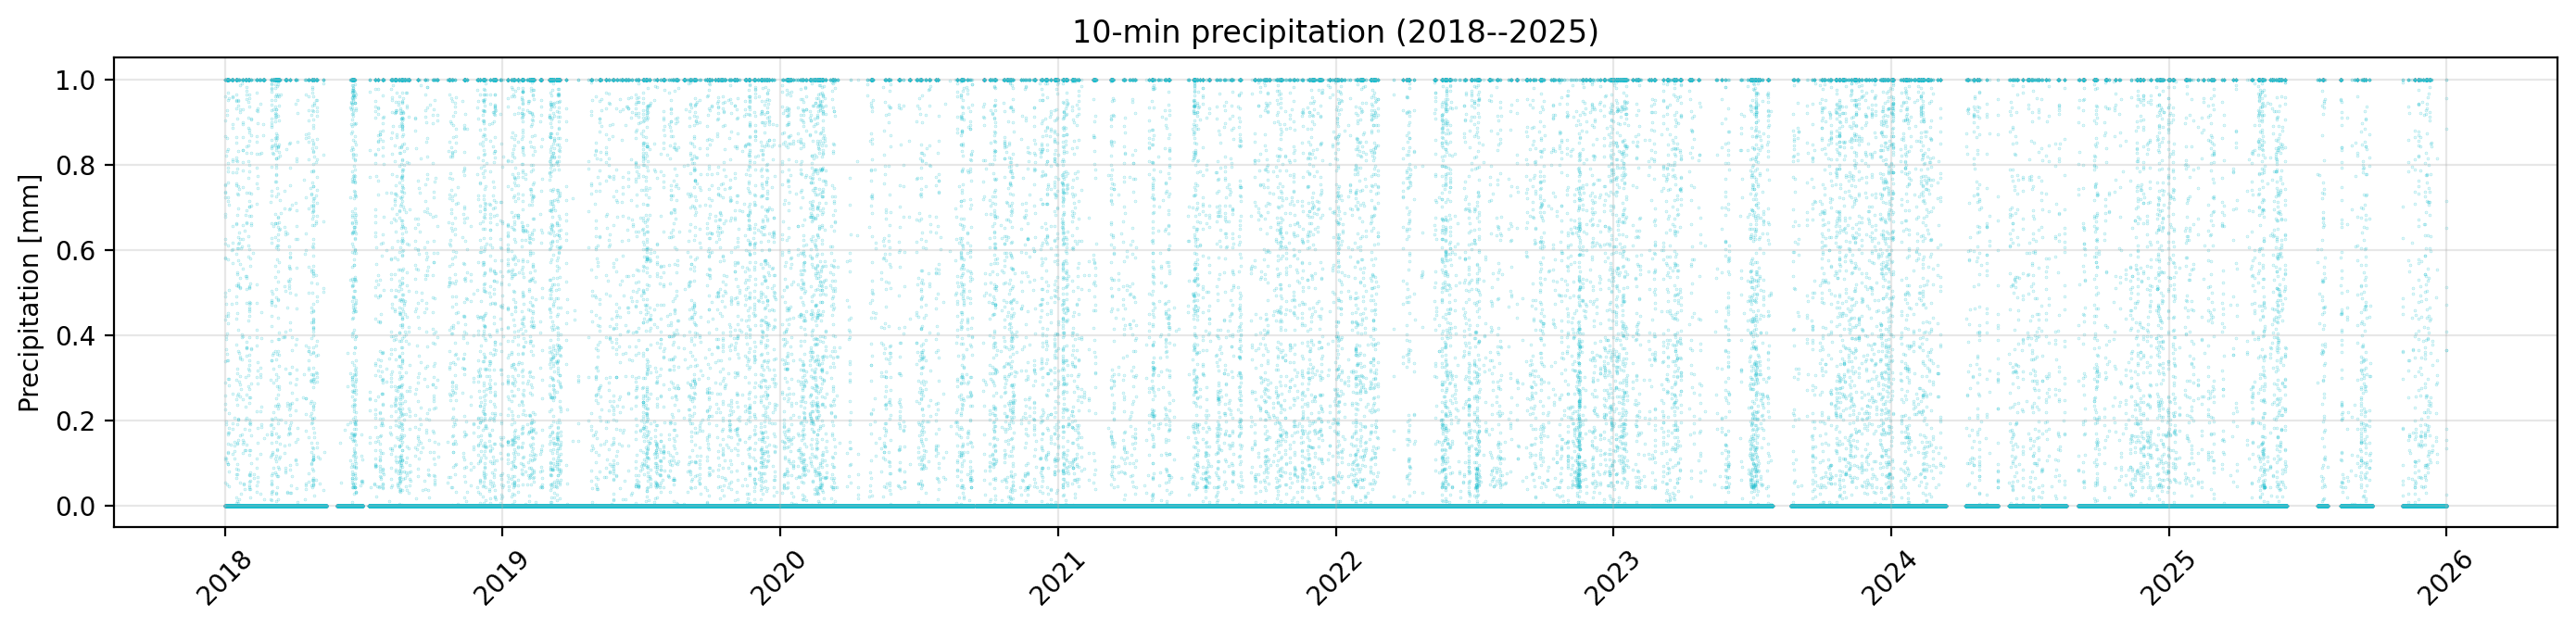
\includegraphics[width=1\textwidth]{figures/Q10_Rain.png}
    \caption{Time series of 10-minute precipitation (Rain) levels across the measurement period.}
\end{figure}

\subsubsection{Data Gap Analysis and Discussion}
To further investigate and assess the data quality, time intervals over the expected 10-minute resolution are identified as gaps. The following figures show the temporal distribution and duration of the missing records.

\begin{figure}[H]
    \centering
    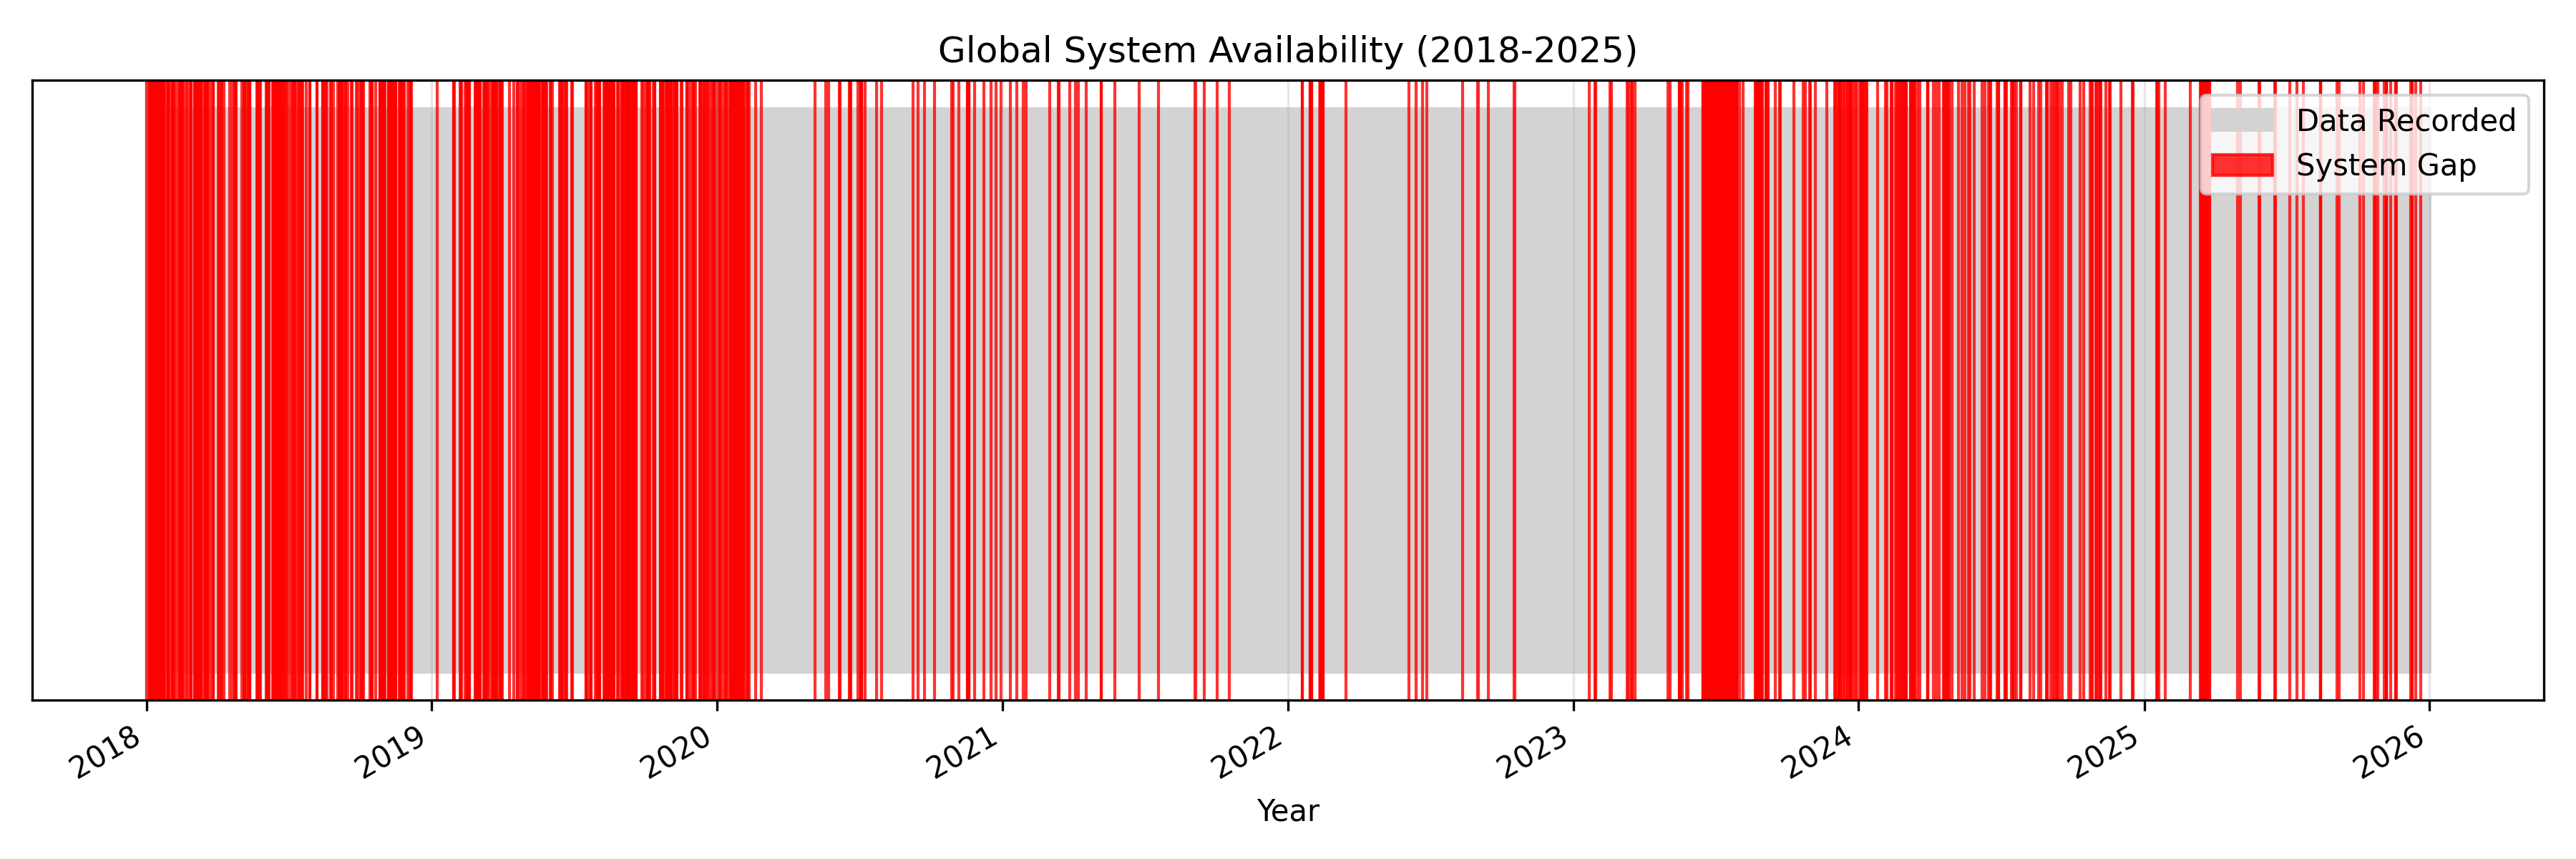
\includegraphics[width=1\textwidth]{figures/Q10_Global_Gaps.png}
    \caption{Global data availability from 2018 to 2026. Red segments identify total system outages where no timestamps were recorded.}
\end{figure}

\begin{figure}[H]
    \centering
    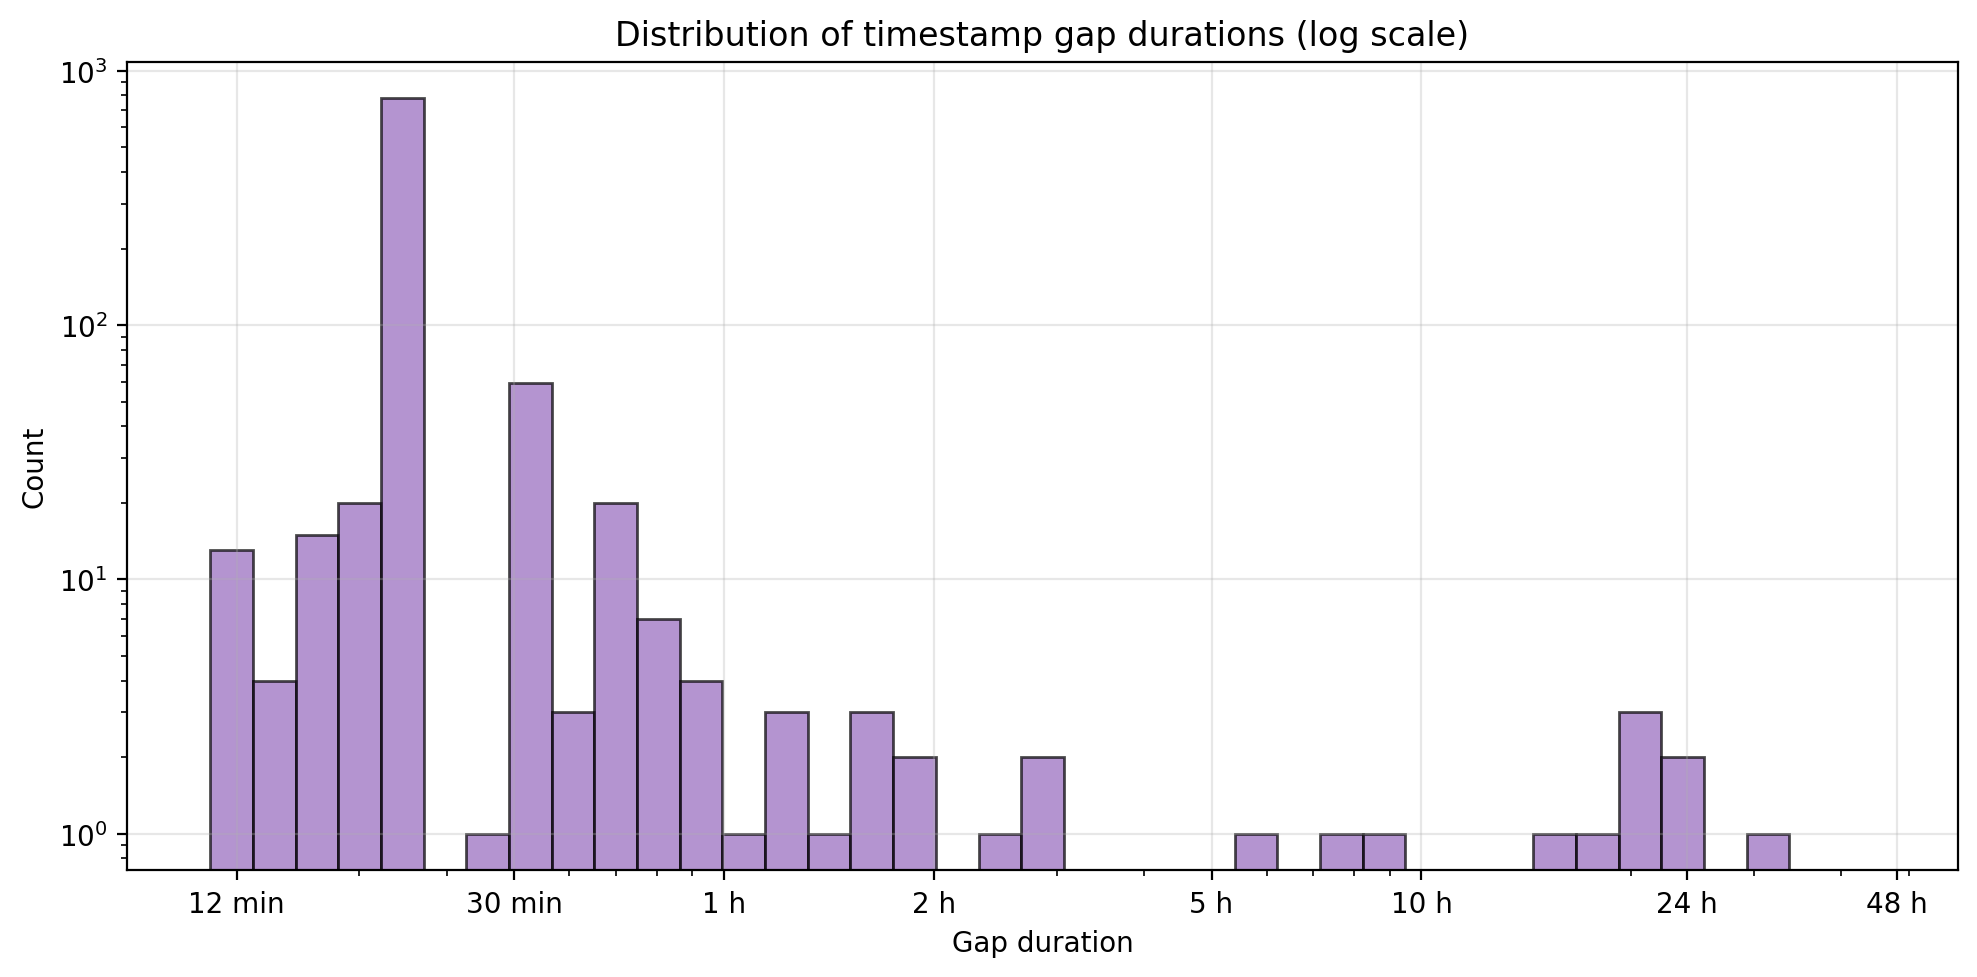
\includegraphics[width=1\textwidth]{figures/Q10_Gap_Histogram.png}
    \caption{Distribution of gap durations on a logarithmic scale, showing the frequency of short versus long-term outages.}
\end{figure}

\begin{figure}[H]
    \centering
    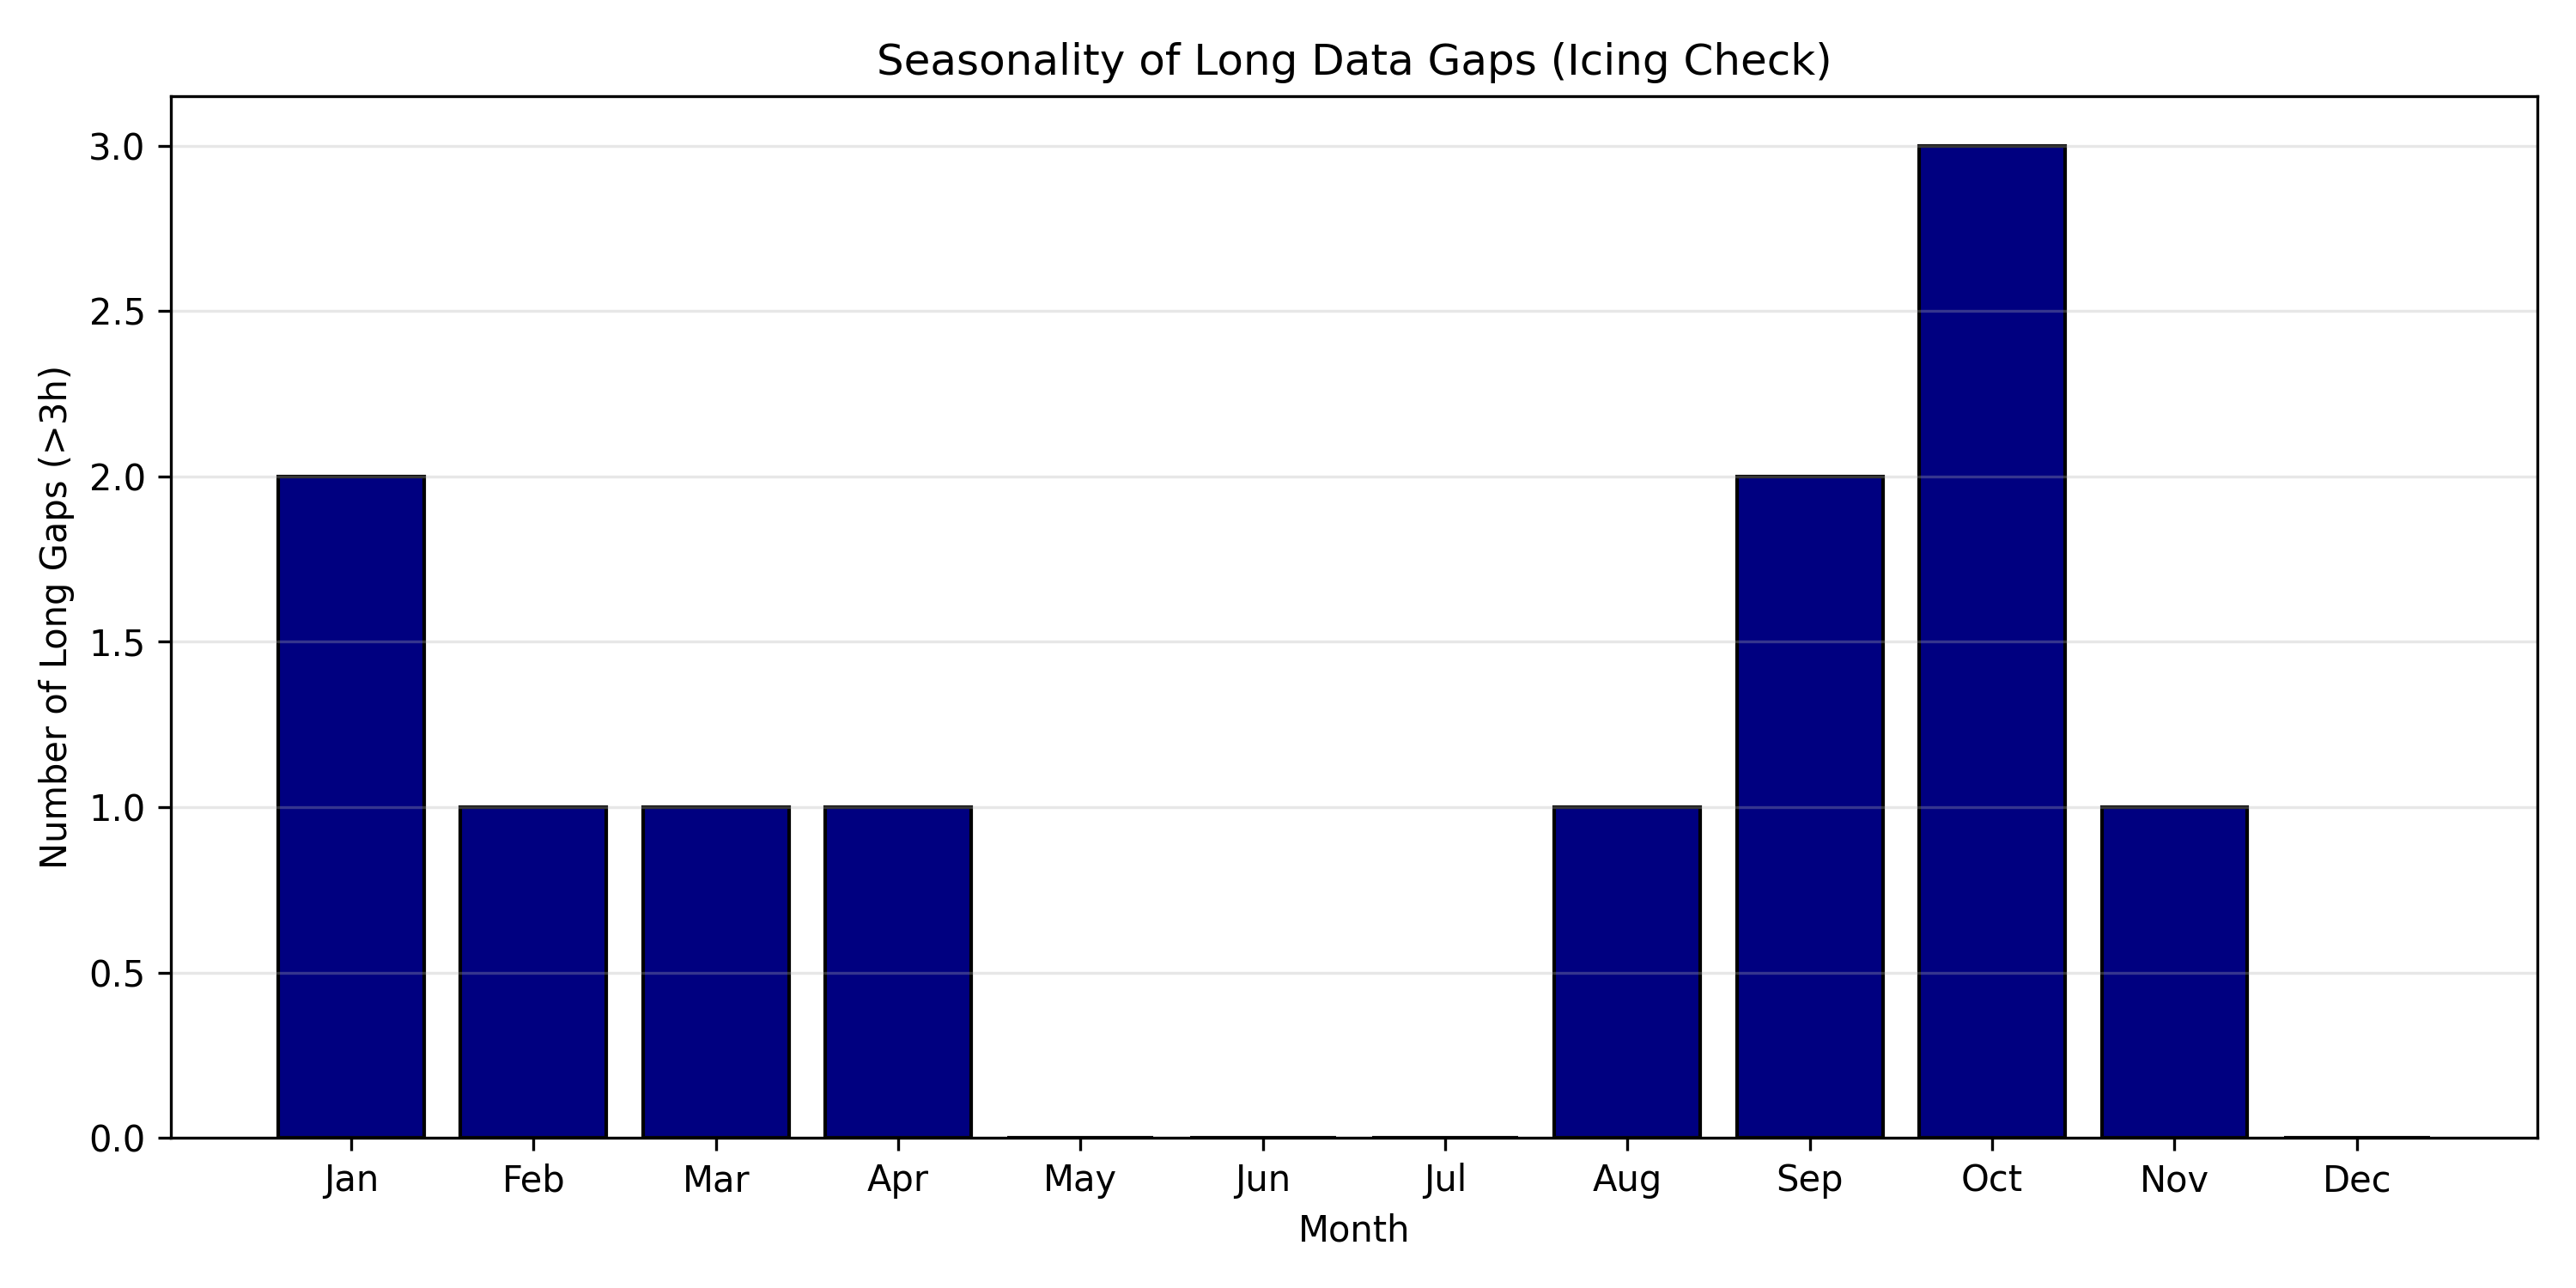
\includegraphics[width=1\textwidth]{figures/Q10_Long_Gap_Seasonality.png}
    \caption{Seasonality of long-term gaps (> 3 hours), highlighting potential periods of sensor icing.}
\end{figure}

\textbf{Discussion of Gaps:}
Possible reasons for the data gaps are:
\begin{itemize}
    \item \textbf{Sensor Icing:} Seasonal analysis shows long-term gaps ($>3$ hours) mainly from January to April. This indicates icing of cup anemometers and ultrasonic paths, which occurs even while the data logger remains powered.
    \item \textbf{Telemetry Errors:} The high frequency of short-duration gaps (10--20 minutes) in the histogram suggests transient signal loss during wireless data transmission from the mast to the server.
    \item \textbf{Local Hardware Defects:} Discrepancies between sensors at different heights (e.g., the 57m direction outage in 2019-2020) point to localized cable damage or specific instrument failure rather than a global system crash.
    \item \textbf{Scheduled Maintenance:} Simultaneous gaps across all sensor channels during summer months are typical for planned annual inspections, sensor calibrations, or manual data retrieval.
    \item \textbf{Atmospheric Interference:} Increased short-term gaps during summer afternoons correlate with lightning activity and electromagnetic interference from storms, potentially triggering automated system reboots.
    \item \textbf{Biological Factors:} Transient blockages of sonic anemometer paths or mechanical interference with cup anemometers by birds can lead to rejected 10-minute averages.
    \item \textbf{Power Supply:} System-wide outages (red bars in the availability plot) may result from battery voltage drops in the solar-powered system during periods of low solar radiation.
\end{itemize}

\subsection{Seasonal Wind Roses}
\textbf{Task:} Using the whole time series, plot a wind rose for the winter months (Dec-Feb) and one for the summer months (Jun-Aug) discuss the directional distribution of the wind. Does it match what you would expect for Denmark?



\subsection{Histogram and Weibull Fit}
\textbf{Task:} Define wind bins with a spacing of 1m/s and plot a histogram of the wind speed variation based on the data from 70m height for two different years, 2018 and 2024. Fit a Weibull distribution to the observed wind speed.

\begin{equation}
    f(u) = \frac{k}{A} \left( \frac{u}{A} \right)^{k-1} \exp\left[ -\left( \frac{u}{A} \right)^k \right]
\end{equation}

\subsection{AEP for V52 Turbine}
\textbf{Task:} Calculate the AEP for the V52 turbine located at the met mast site, based on the 2018 and 2024 wind measured data. Discuss implications on the yearly variability.

\begin{table}[H]
    \centering
    \begin{tabular}{lrr}
        \toprule
        Year & AEP [MWh] & Capacity Factor [\%] \\
        \midrule
        2018 & ... & ... \\
        2024 & ... & ... \\
        \bottomrule
    \end{tabular}
    \caption{Annual Energy Production (AEP) and Capacity Factor for the V52 turbine.}
\end{table}

\newpage
\addcontentsline{toc}{section}{References}
\bibliography{document.bib} 
\bibliographystyle{ieeetr}

\newpage
\appendix

\input{appendix}
\label{ch6}



\end{document}
